\documentclass[aspectratio=169, table]{beamer}

\usepackage{colortbl}
\usepackage{xcolor}
\usepackage{listings}
\usepackage{tikz}
\usetikzlibrary{positioning, arrows.meta, fit}

\usetheme{Pradita}


\usepackage{listings}
\lstdefinestyle{SqlStyle}{
language=SQL,
basicstyle=\ttfamily\footnotesize,
morekeywords={REAL, TEXT, REFERENCES},
keywordstyle=\color{blue},
commentstyle=\color{gray},
stringstyle=\color{red},
breaklines=true,
showstringspaces=false,
tabsize=2,
captionpos=b,
numbers=left,
numberstyle=\tiny\color{gray},
frame=lines,
backgroundcolor=\color{lightgray!10},
comment=[l]{//},
morecomment=[s]{/*}{*/},
commentstyle=\color{gray}\ttfamily,
string=[s]{'}{'},
morestring=[s]{"}{"},
%	stringstyle=\color{teal}\ttfamily,
%	showstringspaces=false
}

\lstdefinelanguage{bash} {
keywords={},
basicstyle=\ttfamily\small,
keywordstyle=\color{blue}\bfseries,
ndkeywords={iex},
ndkeywordstyle=\color{purple}\bfseries,
sensitive=true,
commentstyle=\color{gray},
stringstyle=\color{red},
numbers=left,
numberstyle=\tiny\color{gray},
breaklines=true,
frame=lines,
backgroundcolor=\color{lightgray!10},
tabsize=2,
comment=[l]{\#},
morecomment=[s]{/*}{*/},
commentstyle=\color{gray}\ttfamily,
stringstyle=\color{purple}\ttfamily,
showstringspaces=false
}

% Define Java language style for listings
\lstdefinestyle{JavaScript}{
	language=Java,
	basicstyle=\ttfamily\footnotesize,
	keywordstyle=\color{blue},
	commentstyle=\color{gray},
	stringstyle=\color{red},
	breaklines=true,
	showstringspaces=false,
	tabsize=4,
	captionpos=b,
	numbers=left,
	numberstyle=\tiny\color{gray},
	frame=lines,
	backgroundcolor=\color{lightgray!10},
	comment=[l]{//},
	morecomment=[s]{/*}{*/},
	commentstyle=\color{gray}\ttfamily,
	string=[s]{'}{'},
	morestring=[s]{"}{"},
	%	stringstyle=\color{teal}\ttfamily,
	%	showstringspaces=false
}

\title{\Huge NoSQL and \\
\vspace{10pt}
Semi-structured Data}
\subtitle{IT140704 - Big Data for Business}
%\date[Serial]{Penggunaan Large Language Model untuk Pengajaran}
\author{\textbf{Alfa Yohannis}}
\begin{document}

\frame{\titlepage}


\begin{frame}[fragile]
\frametitle{Contents}
\vspace{20pt}
\begin{columns}[t]
	\column{0.5\textwidth}
	\tableofcontents[sections={1-4}]
	
	\column{0.5\textwidth}
	\tableofcontents[sections={5-20}]
\end{columns}
\end{frame}


\begin{frame}{\hfill}
	\centering
	\Huge{\textbf{Are traditional relational databases enough to handle all types of modern business data – or might there be other solutions?}}
\end{frame}


\section{Introduction}

\begin{frame}{Background}
	\vspace{20pt}
	
	\begin{itemize}
		\item In the digital era, data volume, speed, and variety are growing rapidly, known as the 3Vs.
		
		\item RDBMS have long been standard for structured data but struggle with large, flexible, and highly available data needs.
		
		\item \textbf{NoSQL} emerged to provide flexible schemas, fast read-write, and horizontal scalability, supporting semi-structured data like JSON for web, e-commerce, social media, and IoT.
		
		\item This session explains NoSQL concepts, types like Document and Graph Databases, and their role in modern business systems.
	\end{itemize}
	
\end{frame}


\section{Concept of Semi-Structured Data}

\begin{frame}{Definition and Characteristics}
	\vspace{20pt}
	
	Semi-structured data is not stored in rigid relational table schemas but contains tags or hierarchical structures readable by both machines and humans. Unlike structured data with fixed schemas, semi-structured data allows adding new attributes without changing the overall schema definition.
	
	\vspace{10pt}
	Key characteristics:
	\begin{itemize}
		\item \textbf{Schema-on-read:} schema applied when data is read.
		\item \textbf{Hierarchical and flexible:} supports nested structures.
		\item \textbf{Text-based and key-value:} easy to process and human-readable.
		\item \textbf{Extensible:} new attributes can be added without affecting existing data.
	\end{itemize}
	
\end{frame}

\begin{frame}{Common Formats and Business Relevance}
	\vspace{20pt}
	
	Examples of semi-structured data formats:
	\begin{itemize}
		\item \textbf{JSON (JavaScript Object Notation)}
		\item \textbf{XML (eXtensible Markup Language)}
		\item \textbf{YAML (YAML Ain't Markup Language)}
	\end{itemize}
	
	\vspace{10pt}
	Business relevance:
	\begin{itemize}
		\item Supports data integration from various sources without complex transformation.
		\item Accelerates digital application development with dynamic schemas.
		\item Enables processing of unstructured and semi-structured data in big data analytics.
	\end{itemize}
	
\end{frame}

\begin{frame}[fragile]{Example: Product Data in JSON}
	\vspace{20pt}
	
	Example of product data structure in JSON format:
	
	\begin{lstlisting}[style=JavaScript, basicstyle=\ttfamily\scriptsize]
		{
			"id": 101,
			"name": "ASUS VivoBook Laptop",
			"category": "Electronics",
			"price": 8500000,
			"specs": {
				"processor": "Intel i5",
				"ram": "8GB",
				"storage": "512GB SSD"
			},
			"tags": ["laptop", "asus", "notebook", "electronics"]
		}
	\end{lstlisting}
	
	\vspace{5pt}
	JSON supports nested objects (specs) and arrays (tags), enabling seamless integration between services via RESTful APIs.
	
\end{frame}

\section{Introduction to NoSQL}

\begin{frame}{Definition and Business Motivation}
	\vspace{20pt}
	
	\textbf{NoSQL} (Not Only SQL) refers to non-relational database technologies designed to overcome RDBMS limitations in handling modern data challenges. NoSQL stores data in various formats: e.g., JSON docs, key-value pairs, graphs, and wide-column stores.
	
	\vspace{10pt}
	There are four main motivations for NoSQL adoption:
	\begin{itemize}
		\item \textbf{Scalability:} supports horizontal scaling across multiple servers (sharding), ideal for social media and IoT applications.
		\item \textbf{Flexibility:} schema-less structure enables agile development without complex migrations.
		\item \textbf{High performance and availability:} optimised for low latency and high throughput in real-time analytics and streaming.
		\item \textbf{Handling semi-structured and unstructured data:} stores JSON, XML, text, images, and videos more naturally than relational normalisation.
	\end{itemize}
	
\end{frame}

\begin{frame}{Business Drivers for NoSQL Adoption}
	\vspace{20pt}
	
	Key business drivers for adopting NoSQL include:
	
	\vspace{10pt}
	\begin{itemize}
		\item \textbf{Faster innovation and time-to-market:} enables rapid feature development without redesigning rigid schemas.
		\item \textbf{Support for global distributed applications:} databases like Cassandra and DynamoDB replicate data across regions with high availability.
		\item \textbf{Cost efficiency:} scale-out with commodity hardware is more economical than expensive scale-up servers.
	\end{itemize}
	
	\vspace{10pt}
	However, NoSQL does not completely replace RDBMS. Choosing database technology requires evaluating trade-offs between \textbf{Consistency}, \textbf{Availability}, and \textbf{Partition Tolerance} based on the CAP theorem.
	
\end{frame}

\begin{frame}{Main NoSQL Categories (Overview)}
	\vspace{20pt}
	
	NoSQL databases are classified into four main categories:
	
	\begin{itemize}
		\item \textbf{Document Database:} stores data as JSON/BSON documents with dynamic schemas, ideal for user profiles and product catalogues.
		\item \textbf{Key-Value Store:} stores simple key-value pairs, providing high read/write performance for caching and session management.
		\item \textbf{Column-Family Store:} wide-column tables with flexible columns, suitable for large-scale analytics and time-series data.
		\item \textbf{Graph Database:} stores nodes and edges to represent complex relationships, ideal for social networks and fraud detection.
	\end{itemize}
	
\end{frame}

\begin{frame}{NoSQL Categories: Business Use Cases}
	\vspace{20pt}
	
	\begin{table}[h]
		\centering
		\renewcommand{\arraystretch}{1.3}
		\setlength{\tabcolsep}{3pt}
		\footnotesize
		\arrayrulewidth=0.5pt
		\arrayrulecolor{gray}
		
		\begin{tabular}{|p{0.18\textwidth}|p{0.22\textwidth}|p{0.20\textwidth}|p{0.30\textwidth}|}
			\hline
			\textbf{Category} & \textbf{Data Structure} & \textbf{Example DBMS} & \textbf{Business Use Case} \\ \hline
			Document Store & JSON/BSON documents & MongoDB, CouchDB & E-commerce catalogues, user profiles, CMS \\ \hline
			Key-Value Store & Key-value pairs & Redis, DynamoDB & Session store, caching, shopping carts \\ \hline
			Column-Family Store & Wide-column tables & Cassandra, HBase & Time-series, IoT sensor data, big data analytics \\ \hline
			Graph Database & Nodes and edges & Neo4j, Amazon Neptune & Social networks, recommendations, fraud detection \\ \hline
		\end{tabular}
		
		\arrayrulecolor{black} % Reset to default if needed later
	\end{table}
	
	\vspace{10pt}
	Each NoSQL type has advantages suited to specific data characteristics, query patterns, and business goals.
	
\end{frame}

\section{Document Databases}

\begin{frame}{Concept and Structure}
	\vspace{20pt}
	
	\textbf{Document databases} are NoSQL types that store data as semi-structured documents, commonly using \textbf{JSON}, \textbf{BSON}, or XML formats. Each document contains key-value pairs and may include nested objects or arrays.
	
	\vspace{10pt}
	Key features:
	\begin{itemize}
		\item Each document is equivalent to one record (like a row in RDBMS).
		\item Documents are grouped into \textbf{collections} (similar to tables but without rigid schemas).
		\item Schema-less: documents can have different attributes.
		\item Indexing can be created on fields for fast queries.
	\end{itemize}
	
\end{frame}

\begin{frame}{Document Database Structure Diagram}
	\vspace{20pt}
	
	\begin{figure}
		\centering
		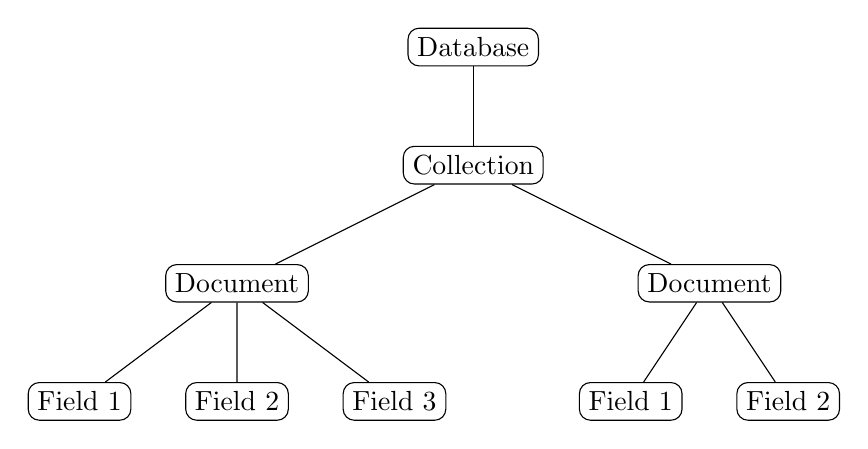
\begin{tikzpicture}[
			node distance=1.2cm,
			every node/.style={rectangle, draw=black, rounded corners, align=center, minimum height=1em},
			level 1/.style={sibling distance=6cm},
			level 2/.style={sibling distance=6cm},
			level 3/.style={sibling distance=2cm}
			]
			\node {Database}
			child { node {Collection}
				child { node {Document}
					child { node {Field 1} }
					child { node {Field 2} }
					child { node {Field 3} }
				}
				child { node {Document}
					child { node {Field 1} }
					child { node {Field 2} }
				}
			};
		\end{tikzpicture}
		\caption{Document Database Structure: Database $\rightarrow$ Collection $\rightarrow$ Document $\rightarrow$ Fields}
	\end{figure}
	
\end{frame}

\begin{frame}[fragile]{Example: MongoDB Product Document}
	\vspace{20pt}
	
	Example of a MongoDB product document in e-commerce:
	
	\begin{lstlisting}[style=JavaScript, basicstyle=\ttfamily\scriptsize]
		{
			"_id": ObjectId("507f1f77bcf86cd799439011"),
			"name": "ASUS VivoBook Laptop",
			"category": "Electronics",
			"price": 8500000,
			"stock": 120,
			"specs": {
				"processor": "Intel i5",
				"ram": "8GB",
				"storage": "512GB SSD"
			},
			"tags": ["laptop", "asus", "notebook", "electronics"]
		}
	\end{lstlisting}
	
\end{frame}

\begin{frame}[fragile]{Example: MongoDB Query}
	\vspace{20pt}
	
	Example query to find electronics products priced below 10 million rupiah:
	
	\begin{lstlisting}[style=JavaScript, basicstyle=\ttfamily\scriptsize]
		db.products.find(
			{ 
				category: "Electronics", 
				price: { $lt: 10000000 } 
			},
			{
				name: 1,
				price: 1,
				category: 1
			}
		);
	\end{lstlisting}
	
	\begin{itemize}
		\item \texttt{db.products.find()}: queries the \texttt{products} collection.
		\item Filter: category Electronics and price < 10 million.
		\item Projection: shows only name, price, and category.
	\end{itemize}
	
\end{frame}

\begin{frame}{Business Use Cases of Document Databases}
	\vspace{20pt}
	
	Document databases are widely used for:
	
	\begin{itemize}
		\item \textbf{Product catalogues}: flexible structures for varied product attributes.
		\item \textbf{User profiles}: dynamic data with preferences, transactions, metadata.
		\item \textbf{Content management systems (CMS)}: storing articles, web pages, digital content.
		\item \textbf{Real-time analytics}: analysing transaction data with evolving schemas.
	\end{itemize}
	
	They enable faster application development, adapting data structures to rapidly changing business needs without sacrificing performance.
	
\end{frame}

\subsection{Comparison: RDBMS vs Document Database for Multi-Category Products}

\begin{frame}[fragile]{RDBMS Approach: Schema-Based}
	\vspace{20pt}
	
	In e-commerce applications with multi-category products (e.g. laptops, books, fashion, furniture), RDBMS requires defining all possible attributes in one table:
	
\begin{lstlisting}[style=SqlStyle]
CREATE TABLE products (id INT PRIMARY KEY, name VARCHAR(100), category VARCHAR(50), price DECIMAL(10,2), screen_size VARCHAR(20), processor VARCHAR(30), ram VARCHAR(20), author VARCHAR(50), page_count INT, material VARCHAR(50), size VARCHAR(30));
\end{lstlisting}

	
	\vspace{5pt}
	\textbf{Limitations:}
	\begin{itemize}
		\item Many columns (e.g. screen\_size, author) are NULL for irrelevant categories.
		\item Adding new categories needs \texttt{ALTER TABLE}, risking downtime.
		\item Queries become inefficient due to irrelevant columns.
		\item Rigid structure slows down agile feature development.
	\end{itemize}
	
\end{frame}

\begin{frame}[fragile]{Document Database Approach: Schema-less}
	\vspace{20pt}
	
	With document databases like MongoDB, each product is stored as a document with category-specific attributes.
	
	\begin{columns}[T]
		
		\column{0.5\textwidth}
		\textbf{Example: Laptop}
\begin{lstlisting}[style=JavaScript, basicstyle=\ttfamily\scriptsize]
{
	"name": "ASUS VivoBook",
	"category": "Electronics",
	"price": 8500000,
	"specs": {
		"screen_size": "15.6 inch",
		"processor": "Intel i5",
		"ram": "8GB"
	}
}
\end{lstlisting}

\column{0.5\textwidth}
\textbf{Example: Book}
\begin{lstlisting}[style=JavaScript, basicstyle=\ttfamily\scriptsize]
{
	"name": "Basic Python Programming",
	"category": "Book",
	"price": 95000,
	"author": "Budi Santoso",
	"page_count": 320
}
\end{lstlisting}

\end{columns}
	
\end{frame}



\begin{frame}{Advantages, Limitations, and Conclusion}
	\vspace{20pt}
	
	\begin{columns}[T]
		
		\column{0.55\textwidth}
		\textbf{Advantages:}
		\begin{itemize}
			\item No empty columns – only relevant attributes stored.
			\item Flexible – new categories/attributes need no schema change.
			\item Efficient nested field queries with indexing.
			\item Developer-friendly – aligns with JSON-based app data.
			\item Supports fast changes for dynamic business needs.
		\end{itemize}
		
		\column{0.45\textwidth}
		\textbf{Limitations:}
		\begin{itemize}
			\item Weak multi-document transaction support.
			\item No global integrity constraints; handled in app logic.
			\item Limited cross-collection joins; complex aggregations require multiple queries or embedding.
			\item Storage overhead with large nested documents.
		\end{itemize}
	\end{columns}
\vspace{10pt}
Document databases like MongoDB excel in flexibility and rapid development, while RDBMS remain optimal for strict ACID transactions and relational integrity.
\end{frame}

\begin{frame}{ACID in RDBMS}
	\vspace{20pt}
	
	\textbf{ACID} is a set of properties ensuring reliable database transactions:
	
	\begin{itemize}
		\item \textbf{Atomicity:} All operations in a transaction succeed or none apply.
		\item \textbf{Consistency:} Transactions bring the database from one valid state to another, maintaining data integrity.
		\item \textbf{Isolation:} Concurrent transactions do not interfere; intermediate states are invisible to others.
		\item \textbf{Durability:} Once committed, transaction changes persist even during system failures.
	\end{itemize}
	
	These properties ensure data reliability and integrity in business-critical applications such as banking, ERP, and accounting systems.
	
\end{frame}


\section{Graph Databases}

\begin{frame}{Graph Database Concept and Structure}
	\vspace{20pt}
	
	\textbf{Graph databases} are NoSQL types designed to store and manage highly connected data with complex relationships.
	
	\vspace{10pt}
	Key components:
	\begin{itemize}
		\item \textbf{Node:} represents entities (e.g. user, product, account).
		\item \textbf{Edge:} represents relationships between nodes, such as “buys”, “friends with”, “recommends”.
		\item \textbf{Properties:} attributes of nodes or edges, e.g. name, age, price, date.
	\end{itemize}
	
	Unlike relational databases that use tables and joins, graph databases store relationships directly, enabling fast traversal without complex join operations.
	
\end{frame}

\begin{frame}{Advantages of Graph Databases}
	\vspace{20pt}
	
	Main advantages include:
	
	\begin{itemize}
		\item Optimised for complex relationship queries and multi-hop traversal.
		\item Stores relationships directly without joins, making connected data queries efficient.
		\item Flexible – new node or relationship types can be added without global schema changes.
	\end{itemize}
	
	These benefits make graph databases ideal for applications where relationships are as important as the data itself.
	
\end{frame}

\begin{frame}{Graph Database Structure Example}
	\vspace{20pt}
	
	\begin{figure}
		\centering
		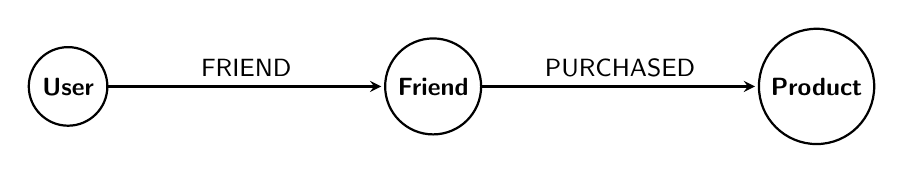
\begin{tikzpicture}[->,>=stealth,shorten >=1pt,auto,
			thick,main node/.style={circle,draw,font=\sffamily\small\bfseries}]
			
			\node[main node] (1) {User};
			\node[main node] (2) [right=3.5cm of 1] {Friend};
			\node[main node] (3) [right=3.5cm of 2] {Product};
			
			\path[every node/.style={font=\sffamily\small}]
			(1) edge node [above] {FRIEND} (2)
			(2) edge node [above] {PURCHASED} (3);
		\end{tikzpicture}
		\caption{Graph Database Structure: User $\rightarrow$ Friend $\rightarrow$ Product for recommendation}
	\end{figure}
	
\end{frame}

\begin{frame}[fragile]{Example: Cypher Query in Neo4j}
	\vspace{20pt}
	
	\textbf{Neo4j} is the most popular graph database, using the property graph model with Cypher Query Language (CQL).
	
	Example query to recommend products purchased by a user’s friends:
	
	\begin{lstlisting}[style=SqlStyle, basicstyle=\ttfamily\scriptsize]
		MATCH (user:User)-[:FRIEND]->(friend:User)-[:PURCHASED]->(product:Product)
		WHERE user.name = "Andi"
		RETURN DISTINCT product.name;
	\end{lstlisting}
	
	This query finds products purchased by friends of “Andi” for personalised recommendations.
	
\end{frame}

\begin{frame}{Business Use Cases}
	\vspace{20pt}
	
	Graph databases are widely used for:
	
	\begin{itemize}
		\item \textbf{Social networks:} storing friends, followers, interactions.
		\item \textbf{Recommendation engines:} suggesting products based on other users with similar connections.
		\item \textbf{Fraud detection:} detecting suspicious transaction patterns.
		\item \textbf{Knowledge graphs:} connecting entities and concepts to support semantic search.
	\end{itemize}
	
	Their ability to analyse relationships and connection patterns makes graph databases a key foundation in network-based and modern analytics applications.
	
\end{frame}

\subsection{Technical Case Example: Graph Database Advantages}

\begin{frame}{\Large{Scenario: Product Recommendation Based on User Relationships}}
	\vspace{20pt}
	
	\textbf{Scenario.} An e-commerce platform wants to recommend products to users based on purchases by other users with similar preferences or social connections (collaborative filtering).
	
	\vspace{10pt}
	Data structure:
	\begin{itemize}
		\item Users have friendship relationships.
		\item Users purchase products.
		\item Products have categories or features.
	\end{itemize}
	
	This requires querying relationships between users and products efficiently.
	
\end{frame}

\begin{frame}[fragile]{RDBMS Approach: Challenges}
\vspace{20pt}	
\begin{lstlisting}[style=SqlStyle]
CREATE TABLE users (user_id INT PRIMARY KEY, name VARCHAR(100));
CREATE TABLE products (product_id INT PRIMARY KEY, name VARCHAR(100), category VARCHAR(50));
CREATE TABLE purchases (user_id INT, product_id INT,
FOREIGN KEY (user_id) REFERENCES users(user_id),
FOREIGN KEY (product_id) REFERENCES products(product_id));
CREATE TABLE friends (user_id INT, friend_id INT,
FOREIGN KEY (user_id) REFERENCES users(user_id),
FOREIGN KEY (friend_id) REFERENCES users(user_id));
\end{lstlisting}

	\textbf{Limitations:}
	\begin{itemize}
		\item Querying “products purchased by user’s friends” requires multiple joins, becoming complex and slow with large datasets.
		\item Each relationship traversal needs an additional join, increasing SQL query complexity and execution time.
	\end{itemize}
	
\end{frame}

\begin{frame}[fragile]{Graph Database Approach: Neo4j Example}
	\vspace{20pt}
	
	\begin{columns}[T]
		
		\column{0.5\textwidth}
		Using graph databases like Neo4j:
		
		\vspace{5pt}
		\textbf{Node and edge structure:}
		\begin{itemize}
			\item Nodes: User, Product
			\item Edges: FRIEND, PURCHASED
		\end{itemize}
		
		\vspace{5pt}
		\textbf{Example Cypher query:}
\begin{lstlisting}[style=SqlStyle, basicstyle=\ttfamily\scriptsize]
MATCH (user:User)-[:FRIEND]-> 
	(friend:User)-[:PURCHASED]-> 
	(product:Product) 
WHERE user.name = "Andi" 
RETURN DISTINCT product.name;
\end{lstlisting}
		
		\column{0.5\textwidth}
		
		\textbf{Advantages:}
		\begin{itemize}
			\item Fast multi-hop traversal without table joins.
			\item Intuitive data model for user–friend–product relationships.
			\item Optimised for social recommendations, shortest path, community detection.
			\item Scales to millions of nodes and edges with stable performance.
		\end{itemize}
		
	\end{columns}
	
\end{frame}

\begin{frame}{Limitations and Conclusion}
	\vspace{20pt}
	
	\textbf{Limitations:}
	\begin{itemize}
		\item Less optimal for large aggregation queries like monthly sales reports.
		\item High storage overhead for edge-heavy graphs (e.g. dense social networks).
		\item Learning curve for Cypher or Gremlin for teams used to SQL.
		\item Integration with RDBMS data requires ETL pipelines or federated queries, increasing architecture complexity.
	\end{itemize}
	
	\vspace{10pt}
	\textbf{Conclusion.} For complex relationship analysis such as social recommendations, fraud detection, or supply chain network analysis, \textbf{graph databases} are superior to RDBMS or document databases due to their high-performance multi-hop traversal and natural data modelling.
	
\end{frame}

\section{Comparison of NoSQL and RDBMS}

\begin{frame}{NoSQL vs RDBMS: Key Characteristics}
	\vspace{20pt}
	
	\textbf{RDBMS} and \textbf{NoSQL} have different strategic roles in modern data management that can deliver effective and scalable systems.
	
	\vspace{5pt}
	\textbf{Main differences:}
	
	\begin{itemize}
		\item \textbf{Data structure:} RDBMS uses relational tables with fixed schemas; NoSQL supports flexible formats (document, key-value, columnar, graph).
		\item \textbf{Schema:} RDBMS is rigid; NoSQL is flexible (schema-less or schema-later).
		\item \textbf{Query language:} RDBMS uses standard SQL; NoSQL varies (e.g. MQL, CQL).
		\item \textbf{Transactions:} RDBMS supports full ACID; NoSQL is mostly BASE with limited transactions.
		\item \textbf{Scalability:} RDBMS scales vertically; NoSQL horizontally.
		\item \textbf{Use cases:} RDBMS suits OLTP, ERP, CRM; NoSQL fits big data, real-time analytics, IoT, social networks.
	\end{itemize}
	
\end{frame}


\begin{frame}{Advantages and Limitations}
	\vspace{20pt}
	
	\textbf{RDBMS}
	\begin{itemize}
		\item \textbf{Advantages:} Strong data consistency, mature industry standard, supports complex transactions with integrity constraints (e.g. foreign keys).
		\item \textbf{Limitations:} Less flexible for semi-structured data; not optimal for horizontal scaling in distributed systems.
	\end{itemize}
	
	\vspace{10pt}
	\textbf{NoSQL}
	\begin{itemize}
		\item \textbf{Advantages:} High horizontal scalability, flexible schema for semi-structured/unstructured data, ideal for big data and real-time apps.
		\item \textbf{Limitations:} Limited ACID transaction support, varied query languages with learning curve, and eventual consistency trade-offs in systems needing real-time accuracy.
	\end{itemize}
	
\end{frame}

\begin{frame}{Strategic Implications for Business Systems}
	\vspace{20pt}
	
	Choosing between RDBMS and NoSQL has strategic impacts:
	
	\begin{itemize}
		\item \textbf{Transaction integrity:} RDBMS suits apps needing strict consistency (e.g. banking, ERP) with full ACID (Atomicity, Consistency, Isolation, Durability) support.
		\item \textbf{Scalability and speed:} NoSQL excels with large data volumes, low latency, and high parallel access (e.g. social media, e-commerce).
		\item \textbf{Schema flexibility:} NoSQL supports agile development with fast schema changes, ideal for startups and evolving models.
		\item \textbf{Hybrid use:} Many organisations use both – RDBMS for core transactions, NoSQL for caching, analytics, or real-time apps.
	\end{itemize}
	
	\textbf{Conclusion:} Big data drives NoSQL adoption for flexibility and scale, while RDBMS remains key for reliable transactional systems.
	
\end{frame}

\section{Types of Databases and Business Relevance}

\begin{frame}{DB Types: Purpose \& Business Context 1}
	\vspace{20pt}
	
	Choosing the right database type is crucial to ensure information systems support business needs effectively and efficiently.
		
	\begin{itemize}
		\item \textbf{Relational DB (RDBMS):} Structured data with ACID transactions (OLTP, ERP, CRM); ensures data integrity for business operations.
		\item \textbf{Document DB:} Semi-structured data with flexible schema (product catalogues, user profiles); ideal for rapidly changing data models.
		\item \textbf{Key-Value Store:} Simple data with ultra-fast access (caching, sessions); boosts application performance.
		\item \textbf{Column-based DB:} Separate column storage for fast aggregation queries (data warehouse, analytics); supports complex reporting.
		\item \textbf{Graph DB:} Efficient connected data storage (social networks, recommendations, fraud detection); analyses relationships for insights.
	\end{itemize}
	
\end{frame}

\begin{frame}{DB Types: Purpose \& Business Context 2}
	\vspace{15pt}
	
	\begin{itemize}
		\item \textbf{Time-Series DB:} Sequential timestamped data (IoT sensors, financial ticks); enables real-time trend analysis.
		\item \textbf{Search Engine DB:} Text indexing for fast search (full-text, product, documents); improves UX in e-commerce or content platforms.
		\item \textbf{In-Memory DB:} RAM-based storage for ultra-low latency (real-time analytics, gaming leaderboards); supports sub-millisecond response times.
		\item \textbf{Ledger DB:} Immutable transaction storage (financial records, blockchain, audit trails); ensures security and data authenticity.
		\item \textbf{Multi-Model DB:} Supports multiple data models in one system (hybrid apps, data integration); offers high flexibility for combined relational, document, and graph data.
	\end{itemize}
	
	Understanding database types aids strategic decisions in designing data architectures that align with modern business performance, scale, and complexity needs.
	
\end{frame}

\section{Short Case Study}

\begin{frame}{\LARGE{Business Scenario: Multi-Category E-Commerce}}
	\vspace{20pt}
	
	\textbf{Company: Multi-Category E-Commerce}
	
	An e-commerce company sells various products such as electronics, fashion, books, and household items. Their system requires:
	
	\begin{enumerate}
		\item \textbf{Sales Transactions (Order Management)}  
		Recording purchases, payments, and managing product inventory with high data integrity.
		
		\item \textbf{Varied Product Catalogue}  
		Each product category has different attributes (e.g. electronics: CPU, RAM; books: author, pages; fashion: size, colour).
		
		\item \textbf{Product Recommendations Based on Purchase Relationships}  
		Recommending products based on purchases by other users with similar preferences (collaborative filtering).
	\end{enumerate}
	
\end{frame}

\begin{frame}{Database Choices and Analysis}
	\vspace{20pt}
	
	\textbf{Optimal database choice for each need:}
	
	\begin{itemize}
		\item \textbf{Sales Transactions}  
		\textbf{RDBMS (PostgreSQL, MySQL)}  
		- Supports ACID transactions for payments, orders, and stock updates.  
		- Homogeneous data structure with clear table relationships.
		
		\item \textbf{Multi-Category Product Catalogue}  
		\textbf{Document DB (MongoDB)}  
		- Each product can have different attributes without ALTER TABLE.  
		- Supports nested data (e.g. electronic specs).  
		- Flexible for adding new categories or attributes without downtime.
		
		\item \textbf{Product Recommendations}  
		\textbf{Graph DB (Neo4j)}  
		- Efficiently stores and processes user-product relationships.  
		- Supports pattern-based queries (e.g. collaborative filtering).  
		- Optimal for social graph analysis and personalised recommendations.
	\end{itemize}
	
\end{frame}

\begin{frame}{Strategic Recommendation}
	\vspace{20pt}
	
	Based on the analysis, the recommended data architecture is \textbf{polyglot persistence}, using multiple database types to optimise each function:
	
	\vspace{10pt}
	\begin{enumerate}
		\item \textbf{RDBMS} – for sales transactions and financial data integrity (ERP core).
		\item \textbf{Document DB} – for dynamic, heterogeneous product catalogues.
		\item \textbf{Graph DB} – for user-product relationship-based recommendation engines.
	\end{enumerate}
	
	This approach ensures high performance and system agility. Polyglot persistence is a common practice in modern big data architecture to achieve scalability, flexibility, and reliability simultaneously.
	
\end{frame}

\begin{frame}{Other Aspects to Consider in DB Selection}
	\vspace{20pt}
	
	\begin{itemize}
		\item \textbf{Cost and Licensing:} Includes licence fees (commercial vs open-source), operational costs, and total cost of ownership.
		
		\item \textbf{Vendor Lock-In:} Proprietary features may limit migration flexibility and increase switching costs.
		
		\item \textbf{Human Resource Skills:} Availability of staff skilled in the database’s technology stack, learning curves for NoSQL query languages.
		
		\item \textbf{Integration:} Compatibility with existing systems, BI tools, and data pipelines.
		
		\item \textbf{Compliance and Security:} Regulatory requirements, encryption, and audit logging capabilities.
		
		\item \textbf{Community Support:} Active communities provide problem-solving resources, best practices, and third-party tools.
	\end{itemize}
	
	Decisions must align with business objectives, resource capacity, \& long-term IT plans.
	
\end{frame}


\section{Conclusion}

\begin{frame}{Conclusion}
	\vspace{20pt}
	
	\begin{itemize}
		\item Organisations need flexible, scalable data storage in the digital era.
		\item \textbf{NoSQL} complements RDBMS by:
		\begin{itemize}
			\item Handling semi/unstructured data (e.g. JSON, XML).
			\item Supporting low-latency real-time apps.
			\item Scaling horizontally for large transactions or users.
		\end{itemize}
		\item NoSQL types include document, key-value, column-family, and graph databases.
		\item \textbf{RDBMS} excels in high-integrity ACID transactions.
		\item \textbf{NoSQL} offers agility, rapid development, and schema flexibility.
		\item Many organisations use \textbf{polyglot persistence}, combining both to maximise benefits.
		\item Knowing each type’s strengths and limits helps design effective, competitive data architectures.
	\end{itemize}
	
\end{frame}

\end{document}
